\documentclass[border=10pt]{standalone}

\usepackage{tikz}
\usepackage{tikzsymbols}
\usetikzlibrary{calc,patterns,shapes.geometric}

\def\centerarc[#1](#2)(#3:#4:#5){\draw[#1] ($(#2)+({#5*cos(#3)},{#5*sin(#3)})$) arc (#3:#4:#5);}

\begin{document}
	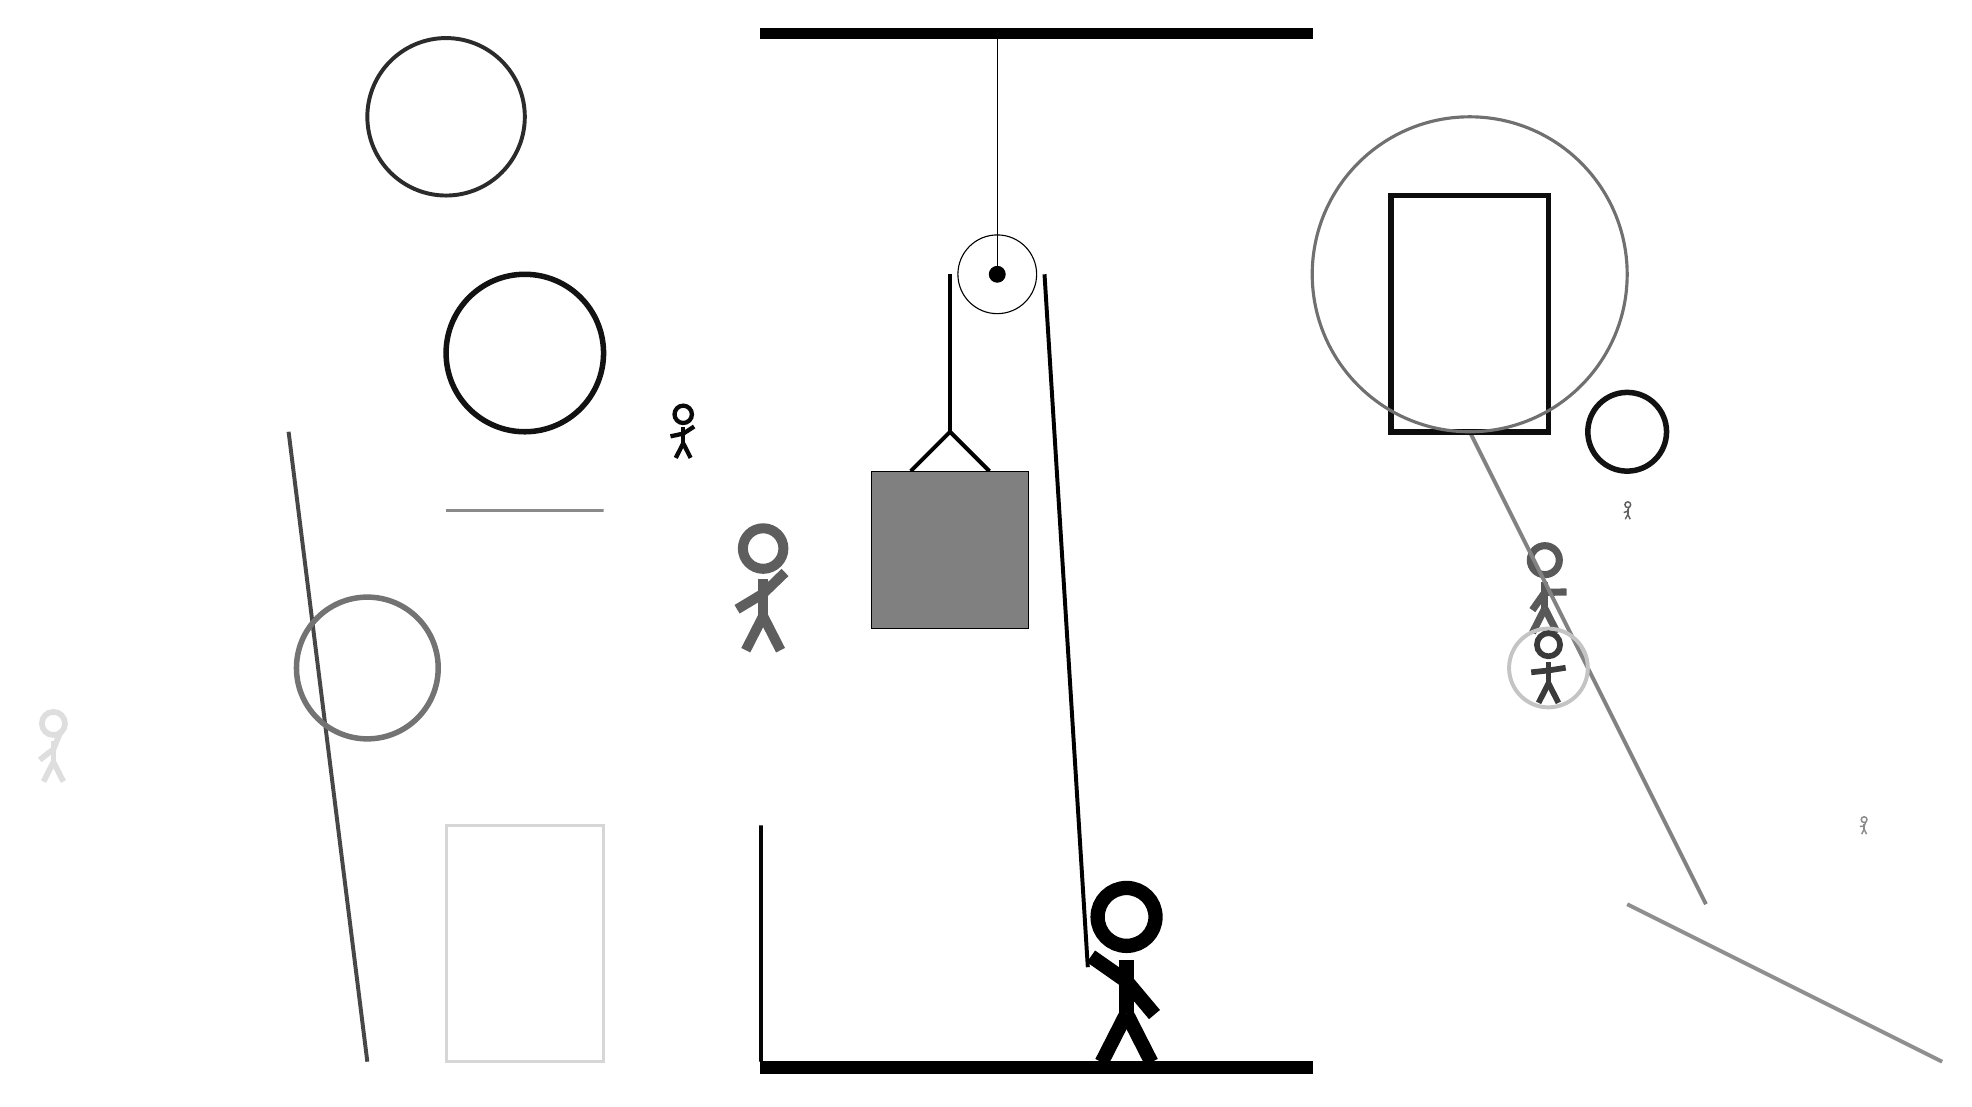
\begin{tikzpicture}
		%%%%% START %%%%%
		
		\draw[fill=black] (-2, 10) rectangle (5, 10.125);
		
		\draw (1, 7) circle (0.5);
		\draw[fill=black] (1, 7) circle (0.1);
		\draw (1, 10) -- (1, 7);
		
		\draw[line width=0.5mm, color=black!44](9, -1) -- (13, -3);
		
		\draw[line width=0.5mm, color=black!72](-7, -3) -- (-8, 5);
		\draw[line width=0.4mm, color=black!16] (-4, -3) rectangle (-6, 0);
		\node[line width=0.4mm, color=black!65] at (8, 3) {\Strichmaxerl[5][55][1]};
		\draw[line width=0.5mm, color=black!49](7, 5) -- (10, -1);
		\draw [line width=0.7mm, color=black!93](-5, 6) circle (1.0);
		\node[line width=0.5mm, color=black!63] at (-2, 3) {\Strichmaxerl[7][31][44]};
		\draw [line width=0.5mm, color=black!83](-6, 9) circle (1.0);
		\node[line width=0.2mm, color=black!46] at (12, 0) {\Strichmaxerl[1][5][68]};
		\node[line width=0.2mm, color=black!96] at (-3, 5) {\Strichmaxerl[3][12][33]};
		\draw [line width=0.7mm, color=black!93](9, 5) circle (0.5);
		\node[line width=0.4mm, color=black!63] at (9, 4) {\Strichmaxerl[1][19][75]};
		\draw[line width=0.7mm, color=black!95] (6, 5) rectangle (8, 8);
		
		\draw [line width=0.4mm, color=black!56](7, 7) circle (2.0);
		\draw [line width=0.5mm, color=black!23](8, 2) circle (0.5);
		\draw[line width=0.5mm, color=black!46] (-4, 4) rectangle (-6, 4);
		
		\draw[line width=0.5mm, color=black!98] (-2, -3) rectangle (-2, 0);
		\node[line width=0.7mm, color=black!13] at (-11, 1) {\Strichmaxerl[4][38][68]};
		\node[line width=0.7mm, color=black!77] at (8, 2) {\Strichmaxerl[4][6][9]};
		\draw [line width=0.7mm, color=black!55](-7, 2) circle (0.9);
		
		\draw[line width=0.5mm] (-0.1, 4.5) -- (0.4, 5.0) -- (0.9, 4.5);
		\draw[fill=black!50] (-0.6, 4.5) rectangle (1.4, 2.5);
		
		\draw[line width=0.5mm] (0.4, 7) -- (0.4, 5.0);
		\centerarc[line width=0.5mm](1, 7)(0:180:0.6);
		\draw[line width=0.5mm](1.6, 7) -- (2.15, -1.8);
		
		\node at (2.6, -1.9) {\Strichmaxerl[10][-35][-50]};
		
		\draw[fill=black] (-2, -3) rectangle (5, -3.15);
		
		%%%%% END %%%%%
	\end{tikzpicture}
\end{document}